\documentclass[international_finance_p2.tex]{subfiles}

\begin{document}
\setbeamercovered{transparent}
\section{Direct Foreign Investment}

\subsection{Direct Foreign Investment}
\begin{frame}{Direct Foreign Investment}
\begin{itemize}[<+->]
\item
Direct foreign investment is the spending by a domestic firm to establish foreign operating units. 
\item
In the balance of payments, direct investment is distinguished from portfolio investment solely on the basis of percentage of ownership.
\item
Capital flows are designated as direct investment when a foreign entity owns 10 percent or more of a firm.
\end{itemize}
\end{frame}
\begin{frame}{Direct investment in Russian Federation}
{in millions of US dollars for years 1994 - 1Q2014}
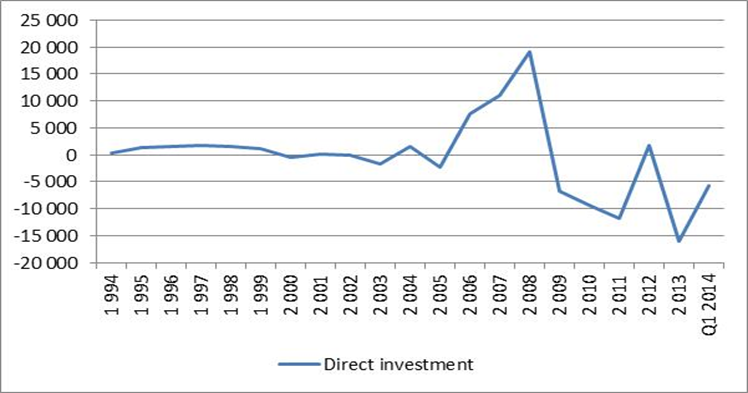
\includegraphics[scale=0.5]{img/fdirus}

Source: Central Bank of Russian Federation, www.cbr.ru. 2014
\end{frame}
\subsection{Capital Flight}
\begin{frame}[shrink=10]{Capital Flight}
\begin{itemize}[<+->]
\item
When the risk of doing business in a country rises sharply or the expected return falls, there are probable large outflows of investment funds so that the country experiences massive capital account deficits.
\item
The change in the risk-return relationship that gives rise to capital flight may be the result of political or financial crisis, tightening capital controls, tax increases, or fear of a domestic currency devaluation.
\item
On the other side, a large capital inflow in a short period of time can lead to an appreciation of the recipient country’s currency. This appreciation may reduce the competitiveness of the nation’s export industries and cause a fall in output and rise in unemployment in these industries.
\end{itemize}
\end{frame}

\subsection{International Lending and Crisis}
\begin{frame}{International Lending and Crisis}
Warning indicators of potential future crises:
\begin{itemize}[<+->]
\item
Fixed exchange rates.
\item
Falling international reserves.
\item
Lack of transparency.
\end{itemize}
\end{frame}

\subsection{IMF Conditionality}
\begin{frame}{IMF Conditionality}
\begin{itemize}[<+->]
\item
The IMF not only “bail out” commercial bank or government creditors. 
\item
The IMF requires borrowers to adjust their economic policies to reduce balance of payments.
\item
The IMF has been criticized for imposing conditions that restrict economic growth and lower living standards in borrowing countries. 
\item
The typical conditionality involves reducing government spending, raising taxes, and restricting money growth.
\end{itemize}
\end{frame}

\subsection{Country Risk Analysis}
\begin{frame}{Country Risk Analysis}
\begin{itemize}[<+->]
\item
The evaluation of the overall political and financial situation in a country and the extent to which these conditions may affect the country’s ability to repay its debts.
\item
There are qualitative and quantitative factors that affect country risk premium
\end{itemize}
\end{frame}
\begin{frame}{Qualitative factors that affect country risk premium}
1. Splits between different language, ethnic, and religious groups that threaten to undermine stability. 

2. Extreme nationalism and aversion to foreigners that may lead to preferential treatment of local interests and nationalization of foreign holdings. 

3. Unfavorable social conditions, including extremes of wealth. 

4. Conflicts in society evidenced by frequency of demonstrations, violence, and guerrilla war.
 
5. The strength and organization of radical groups.
\end{frame}
\begin{frame}{Quantitative factors that affect country risk premium}
1. External debt. 

2. International reserve holdings. 

3. Exports. 

4. Economic growth.
\end{frame}

\end{document}